% SPDX-FileCopyrightText: 2026 Cyprien PIERRE
% SPDX-License-Identifier: CC-BY-4.0
\documentclass[tikz,border=5pt]{standalone}
\usepackage[T1]{fontenc}
\usepackage{lmodern}
\usetikzlibrary{arrows.meta,positioning}
\begin{document}
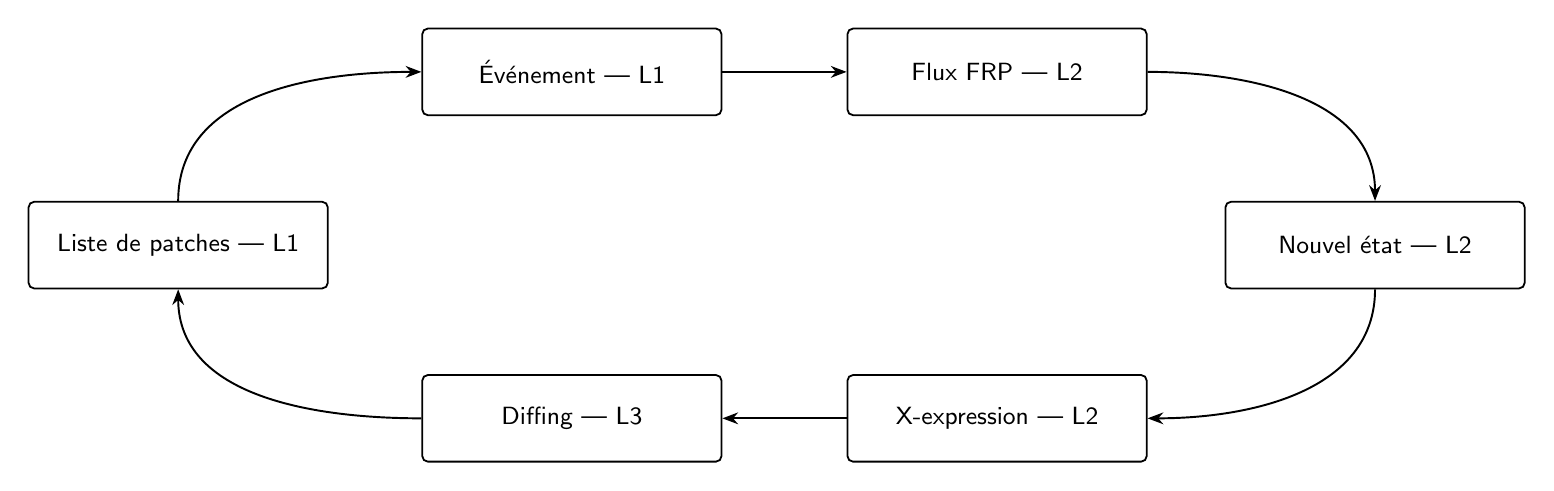
\begin{tikzpicture}[
  font=\sffamily\small,
  box/.style={draw, rounded corners=2pt, align=center, line width=.65pt, minimum height=11mm, minimum width=38mm},
  arrow/.style={-{Stealth[length=2mm]}, line width=.7pt}
]
\node[box] (event) at (58mm,22mm) {Événement --- L1};
\node[box] (flux) at (112mm,22mm) {Flux FRP --- L2};
\node[box] (state) at (160mm,0) {Nouvel état --- L2};
\node[box] (xexpr) at (112mm,-22mm) {X-expression --- L2};
\node[box] (diff) at (58mm,-22mm) {Diffing --- L3};
\node[box] (patches) at (8mm,0) {Liste de patches --- L1};
\draw[arrow] (patches.north) to[out=90, in=180] (event.west);
\draw[arrow] (event) -- (flux);
\draw[arrow] (flux.east) to[out=0, in=90] (state.north);
\draw[arrow] (state.south) to[out=-90, in=0] (xexpr.east);
\draw[arrow] (xexpr) -- (diff);
\draw[arrow] (diff.west) to[out=180, in=-90] (patches.south);
\end{tikzpicture}
\end{document}
